\documentclass[a4paper,12pt]{article}
% \usepackage{libertine}
% \usepackage{libertinust1math}
\usepackage[utf8]{inputenc}
% \usepackage{geometry}
\usepackage{graphicx}
\usepackage{enumitem}
\usepackage{tabs}
\usepackage{amsmath}     
\usepackage{array}
\usepackage{url}
\usepackage[indent=0pt,skip=3mm]{parskip}
\usepackage[top=2cm,bottom=1.5cm]{geometry}
\graphicspath{{D:/code/fisicaComputacional/lab3/images/}}
\newcommand{\eq}[1]{$#1$}
\newcommand{\head}[1]{{\bfseries #1}}
%\setlist{nolistsep}
\setitemize[1]{label=---}
\setenumerate[1]{label=\textcircled{\scriptsize\Alph*},
font=\itshape}

\begin{document}
\title{Metodos de Garlekin y Gauss}
\date{\vspace{-5ex}}
\maketitle
%\tableofcontents
\begin{center}
Escrito por\\
Alván Ventura, Edsel Yael\\ \texttt{ealvan@unsa.edu.pe}
\\[3mm]
Profesor\\Apaza Veliz, Danny Giancarlo\\ \texttt{dapazav@unsa.edu.pe}\\[3mm]
\today
\end{center}
\section{Introducción}
    Los metodos Garlekin y Gauss fueron desarrollados 
    por grandes matematicos como Georgii Ivanovich Petrov, Boris Galerkin y  Carl Friedrich Gauss 
    , quienes propusieron y formaron nuevas formas de solución para ecuaciones discretas,
    sistema de ecuaciones de forma discreta, que en su gran mayoria sirve ahora para
    hacer redes neuronales\cite{5}, modelar ecuaciones diferenciales que a muchas veces
    no tienen una solución analitica. La importancia de estas tecnicas es 
    que pueden ser programadas y de hecho se usan en varias aplicaciones como
    mejorar la resolucion de una imagen tambien llamada "Filtro direccional gaussiano"\cite{1},
    e incluso para resolucion de modelos de programación dinamica.

\section{Metodo Garlekin}
En matemáticas, en el área del análisis numérico, 
los métodos de Galerkin, llamados así por el matemático 
ruso Boris Galerkin, convierten un problema de operador 
continuo, como una ecuación diferencial, comúnmente en 
una formulación débil, en un problema discreto mediante 
la aplicación de restricciones lineales determinadas por 
finito. conjuntos de funciones base.

Fue en honor a Boris Garlekin, que se llamo "Metodos de Garlekin",
estos metodos estan en el campo de análisis numérico, estos metodos toman
un problema continuo, como una ecuación diferencial, en un problema 
discreto mediante la aplicación de restricciones lineales determinadas
por conjuntos finitos.

A continuación se enumeran variaciones del 
Metodo Garlekin:
\begin{enumerate}
    \item \head{Metodo Ritz-Garlekin}:
    normalmente asume una forma bilineal definida simétrica 
    y positiva en la formulación débil, donde la ecuación 
    diferencial para un sistema físico se puede formular 
    mediante la minimización de una función cuadrática que 
    representa la energía del sistema y la solución aproximada 
    es una combinación lineal del conjunto dado de funciones base .
    \item \head{Metodo Bubnov-Galerkin}:
    no requiere que la forma bilineal sea simétrica y 
    sustituye la minimización de energía con restricciones 
    de ortogonalidad determinadas por las mismas funciones 
    de base que se utilizan para aproximar la solución.
    \item \head{Metodo Petrov-Galerkin}:
    Permite utilizar funciones base para restricciones de
    ortogonalidad (llamadas funciones base de prueba) que 
    son diferentes de las funciones base utilizadas para 
    aproximar la solución. El método de Petrov-Galerkin\cite{2} 
    puede verse como una extensión del método de Bubnov-Galerkin, 
    aplicando una proyección que no es necesariamente ortogonal 
    en la formulación del operador de la ecuación diferencial.
\end{enumerate}

En esta monografía, se desarrollara un ejemplo del metodo Petrov-Garleking, concretamente
con el Método de residuos ponderados de Garlekin:
A continuación mostramos la formula que nos ayudara a resolver 
el problema\cite{3}:
%#Mostrar la formula:
\begin{equation}
    \int_{a}^{b} R(x)W_i\,dx = 0
\end{equation}

\subsection{Problema:}
Dada la siguiente ecuación y su respectiva solución analitica,
compruebe usando el metodo de Garlekin una función aproximada.

Ecuacion diferencial:
\begin{equation}
    \frac{\partial^2 y}{\partial x^2} + \frac{\partial y}{\partial x} = 1
\end{equation}

La solucion exacta:
\begin{equation}
    y(x) = 1 - \frac{sen(x)}{sen(1)}
\end{equation}

Las condiciones frontera son:
$$y(0) = 1$$
$$y(1) = 0$$
\newpage
\subsection{Resolución}
A continuación se muestra como se obtiene el polinomio aproximado:
\begin{table}[!ht]
    \centering
    \begin{tabular}{c}
        \begin{minipage}{10cm}
            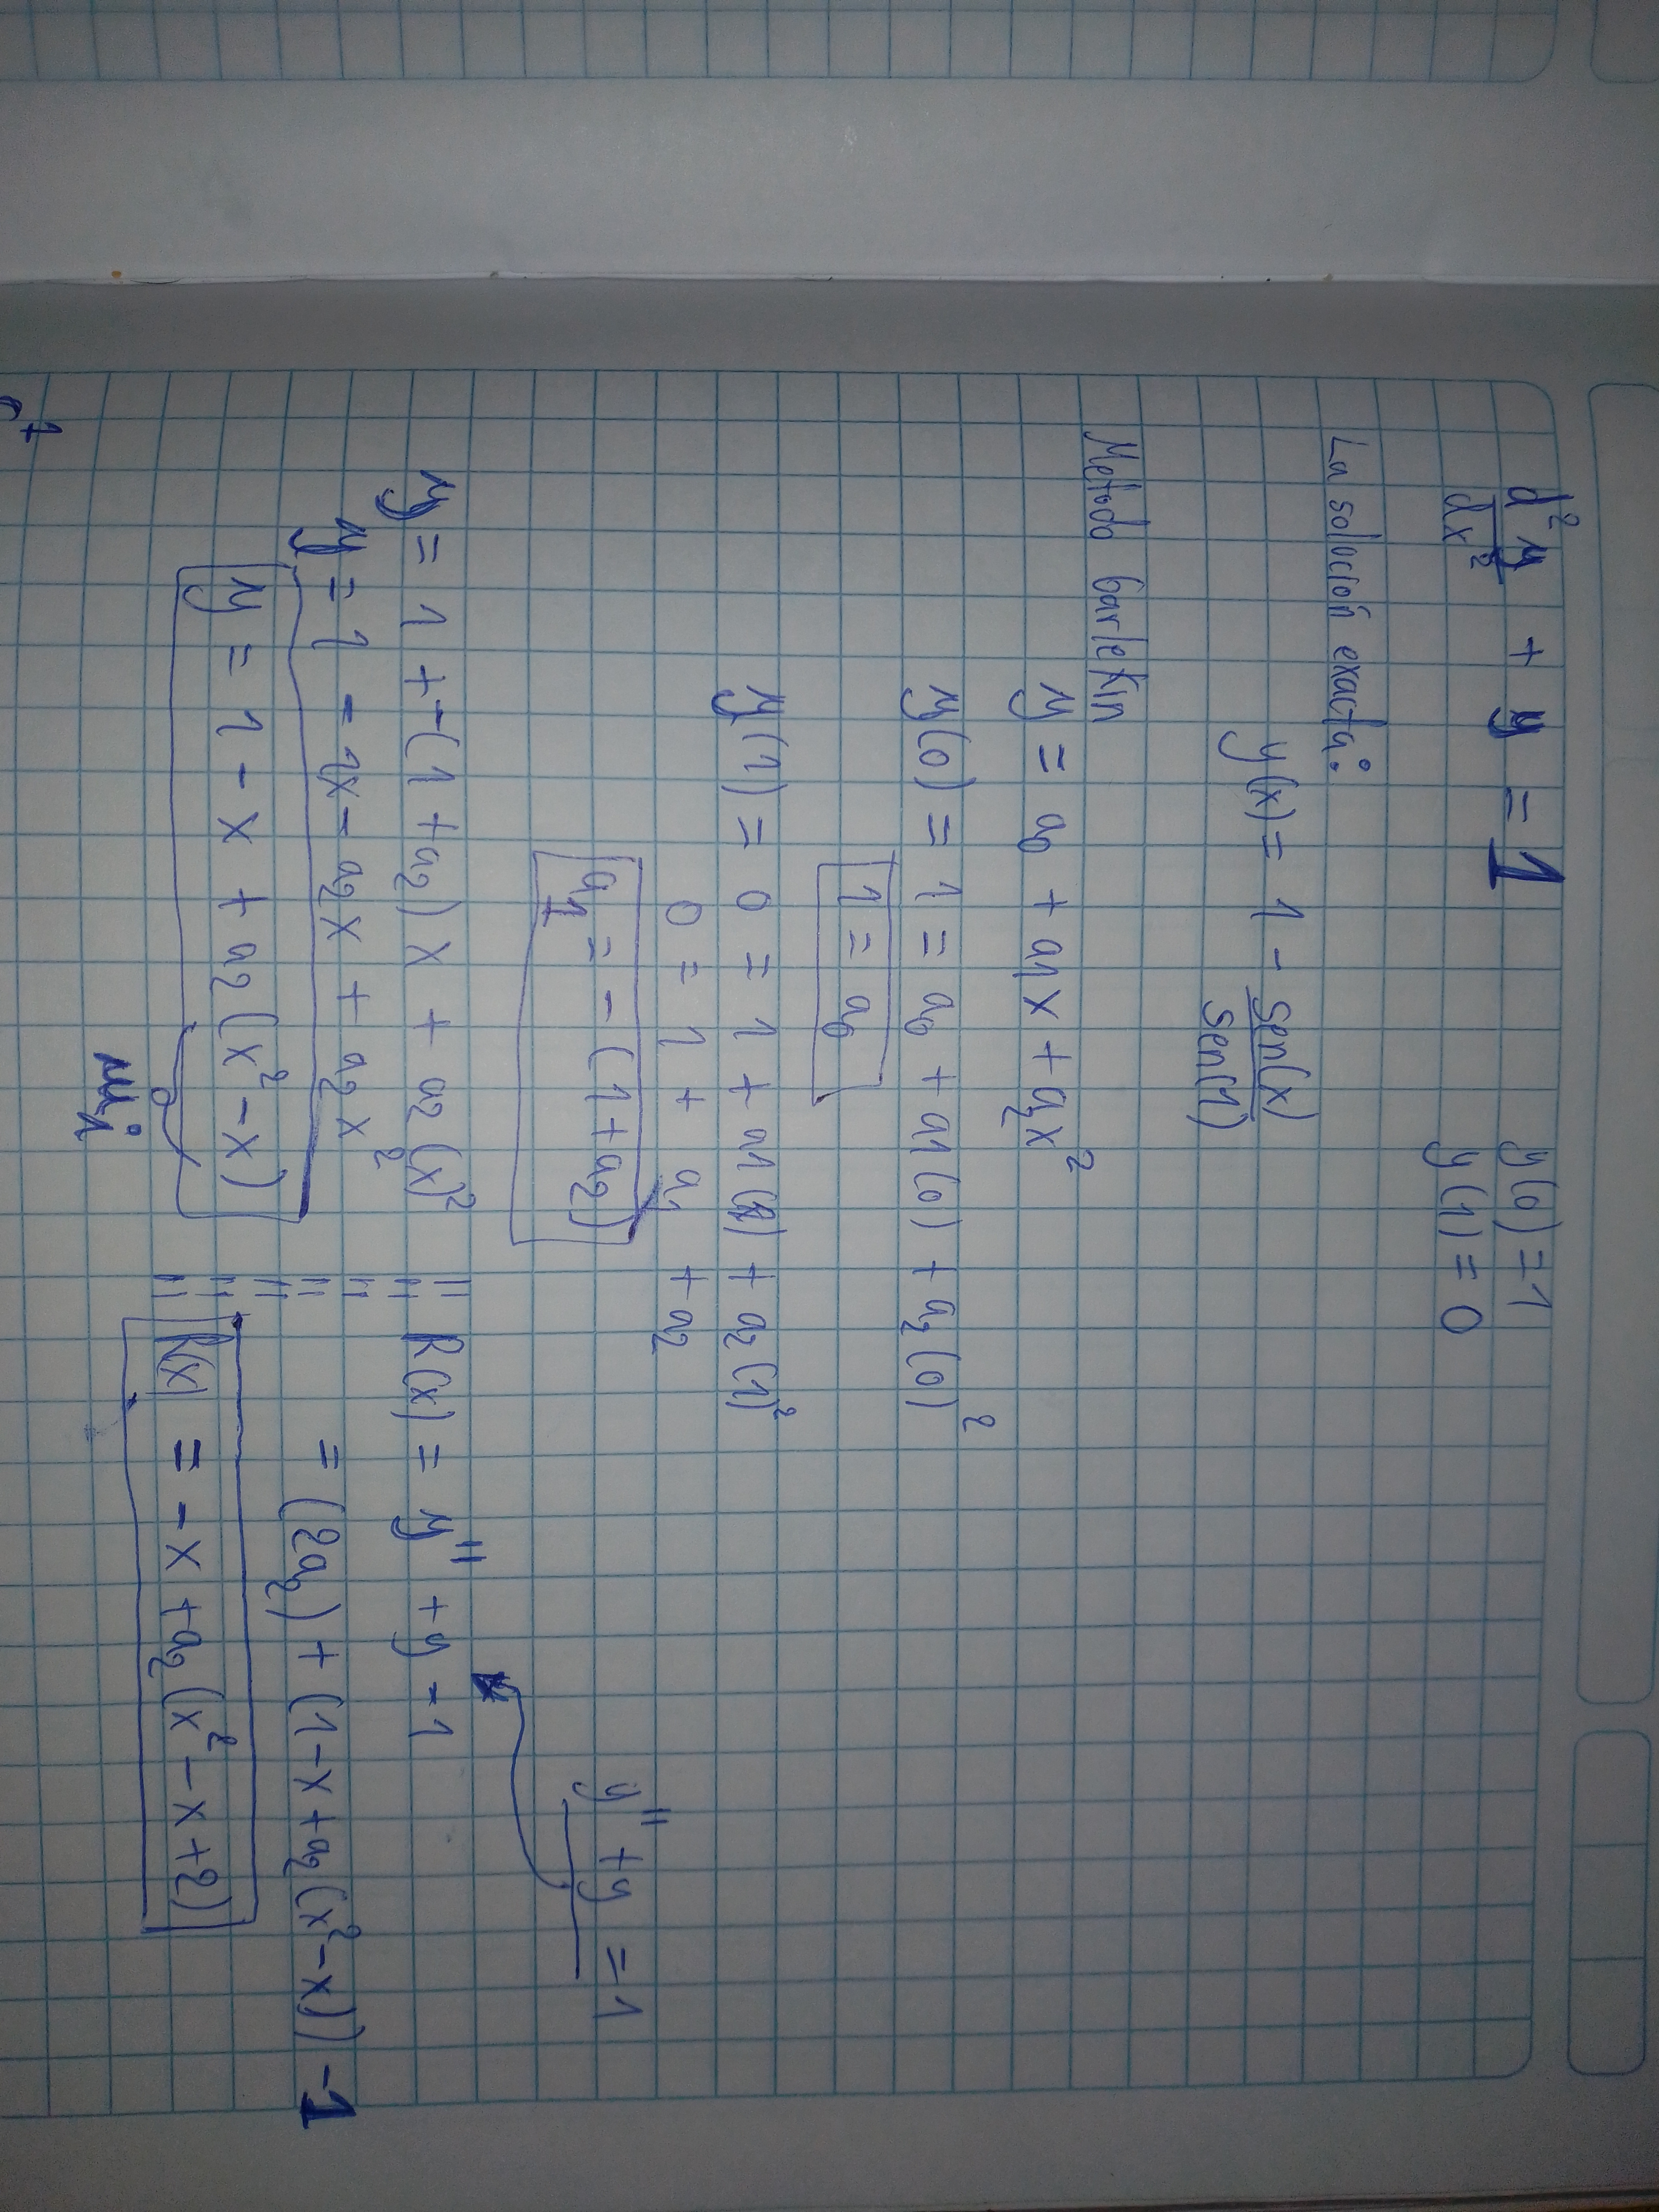
\includegraphics[width=0.7\textwidth,angle=90]{parte1_1}
        \end{minipage}\\
        \begin{minipage}{10cm}
            \includegraphics[width=0.7\textwidth,angle=90]{parte1_2}
        \end{minipage}\\
        \begin{minipage}{10cm}
            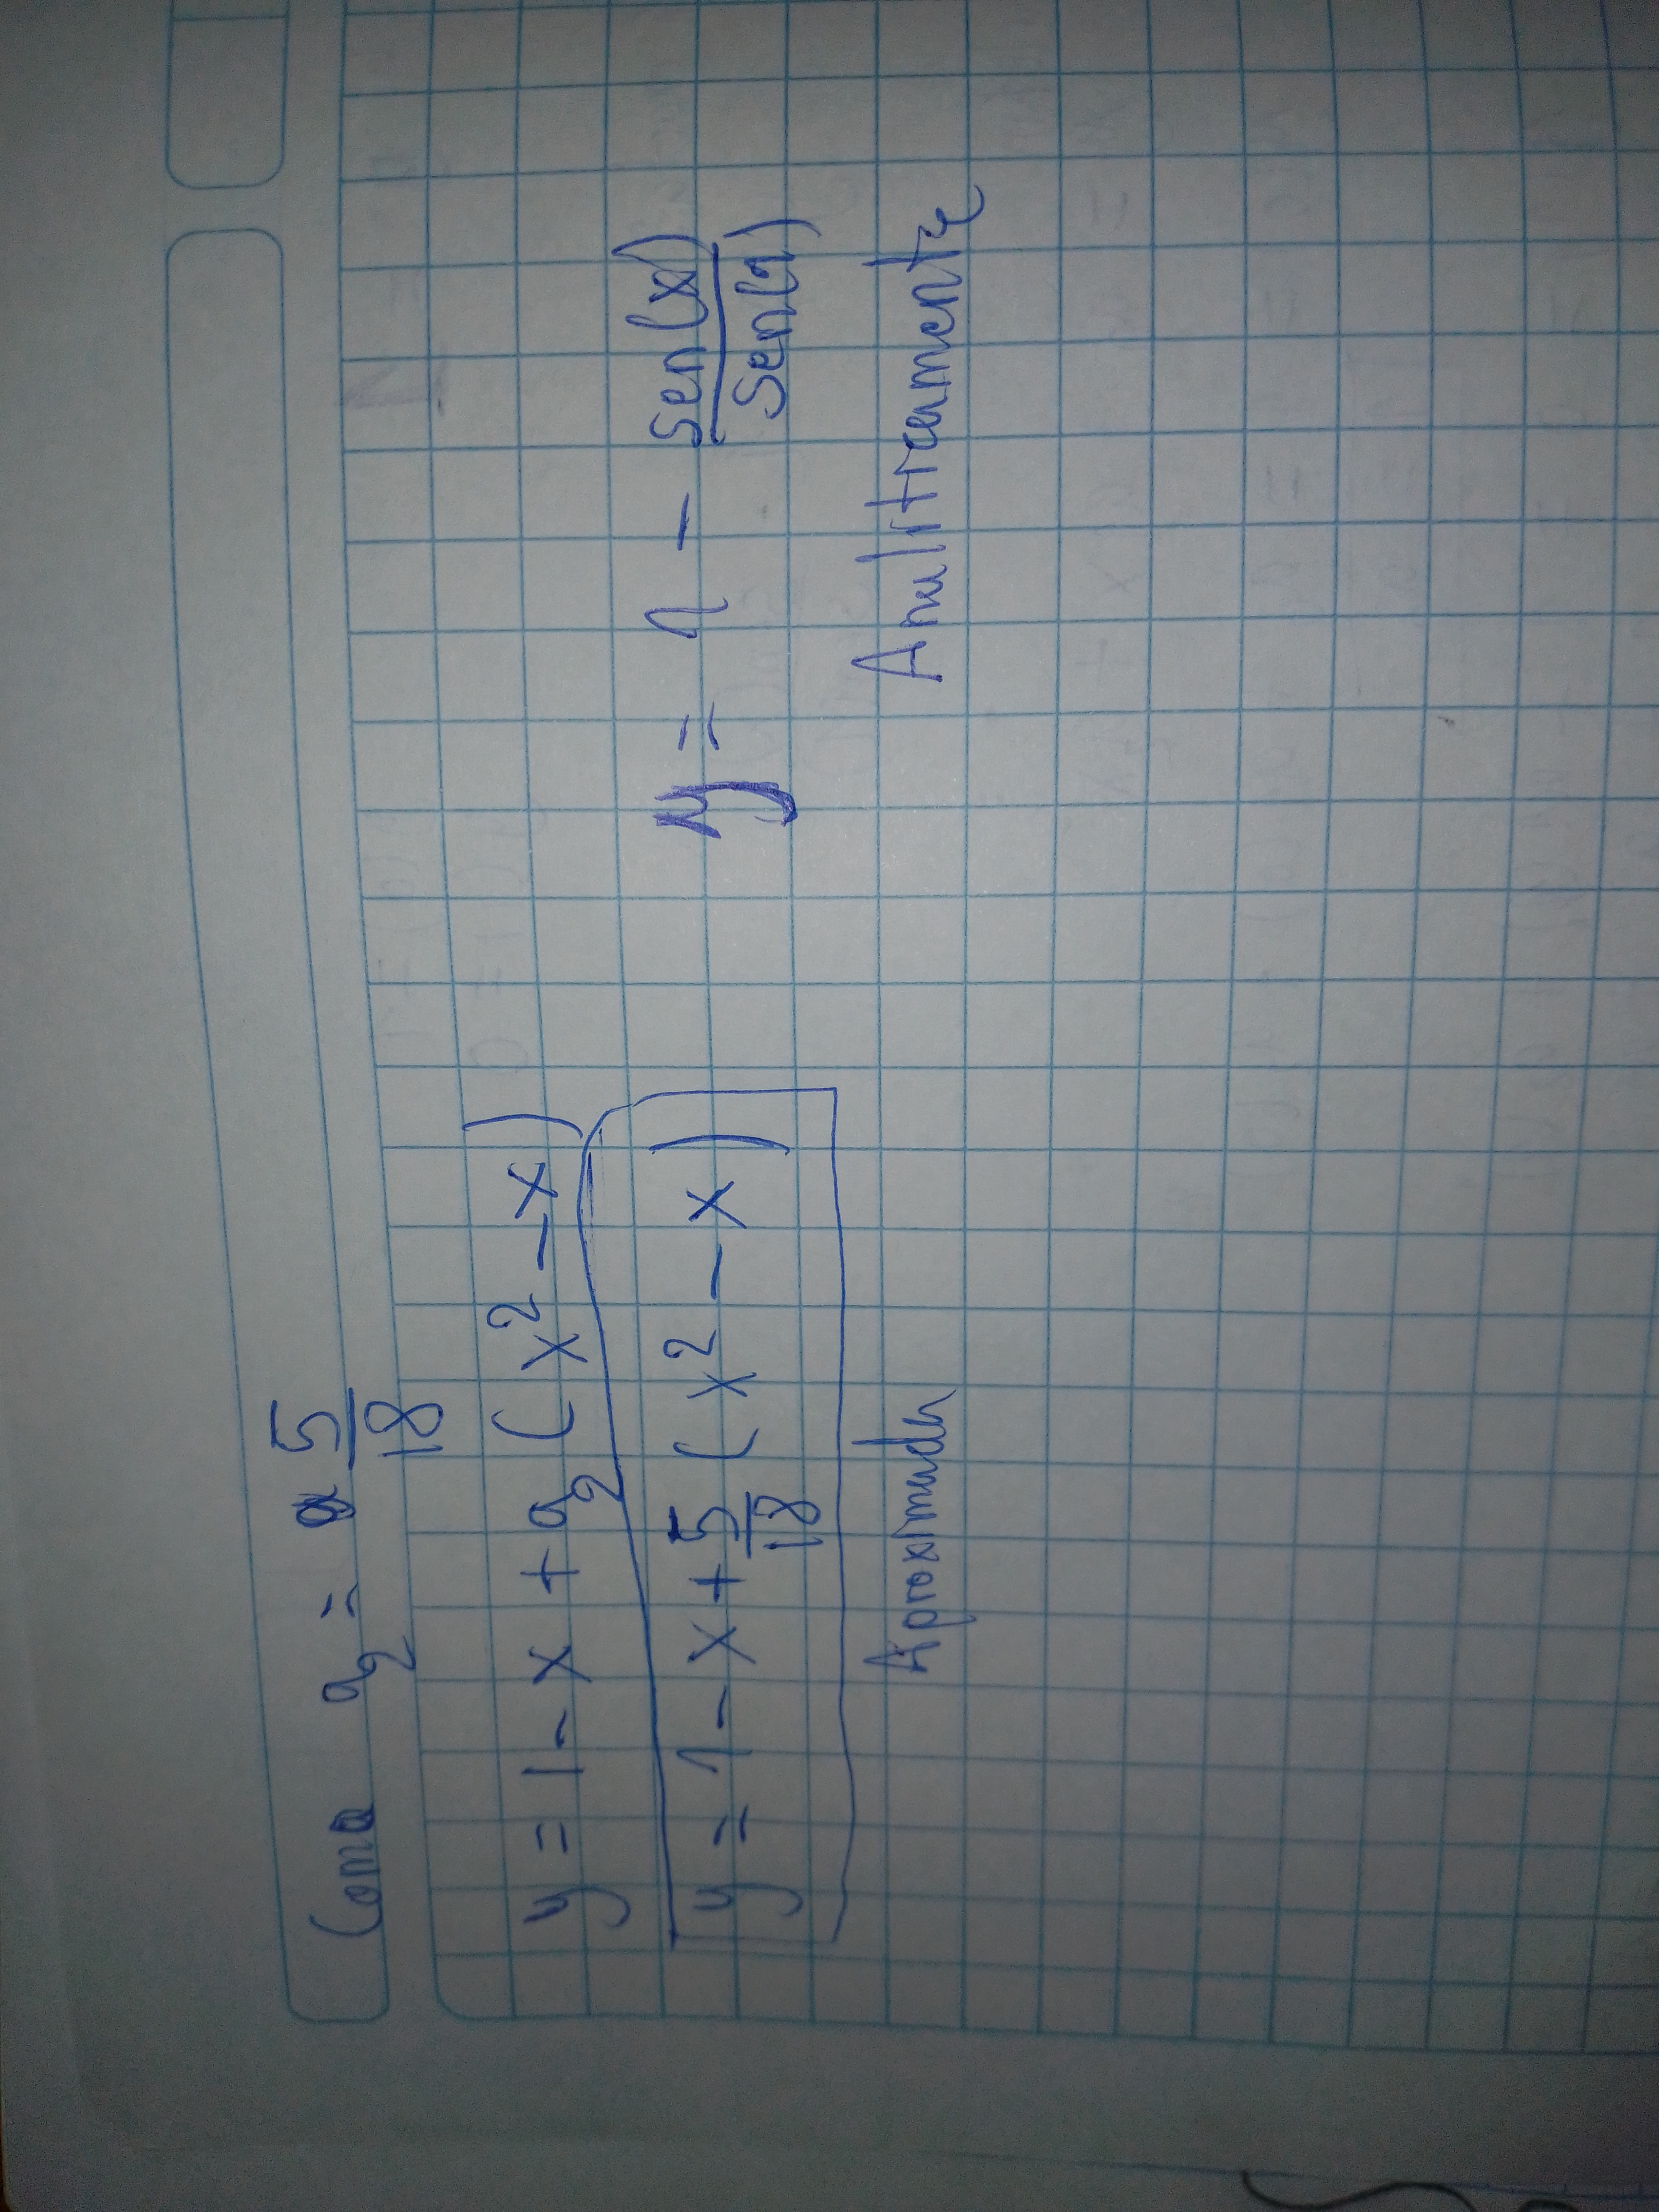
\includegraphics[width=0.7\textwidth,angle=270]{parte1_3}
        \end{minipage}
    \end{tabular}
\end{table}

Y finalmente, nuestro polinomio aproximado es:
\begin{equation}
    y = 1 - x + \frac{5}{18}(x^2 - x)
\end{equation}
% \begin{figure}
%     \centering
%     \includegraphics[scale=0.5]{parte11}
% \end{figure}
% \begin{figure}
%     \centering
%     \includegraphics[scale=0.5]{parte12}
% \end{figure}
\newpage

Ahora veremos en una hoja de excel, como se aproxima los valores
dentro de las condiciones frontera de la numericamente desarrollada con la respuesta analitica:
\begin{figure}[h]
    \centering
    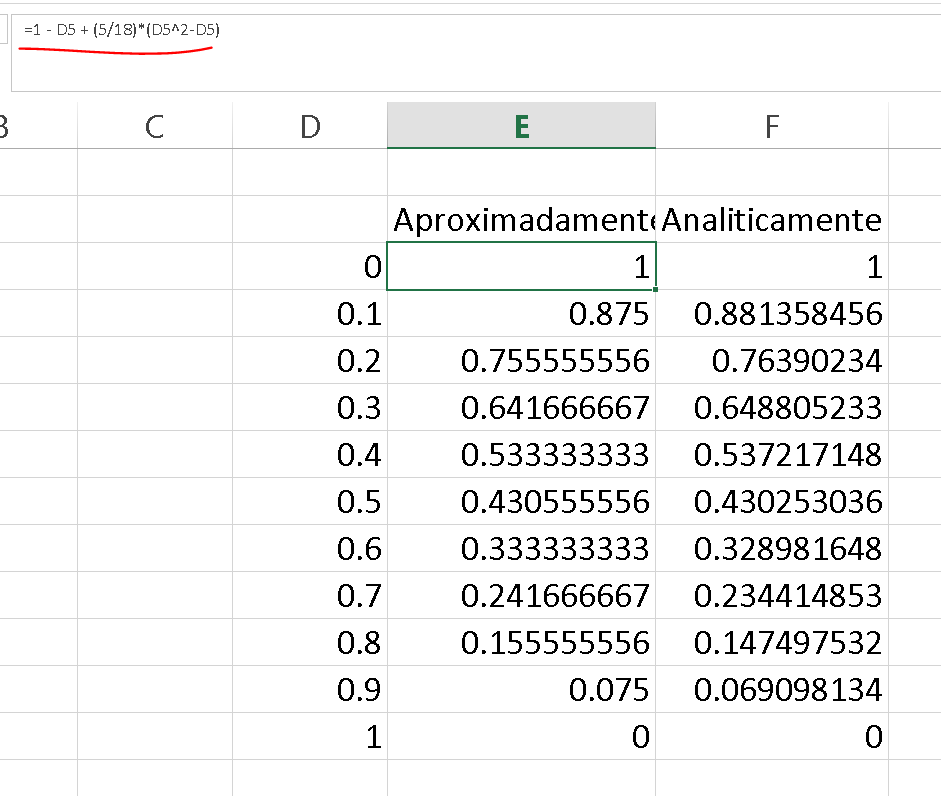
\includegraphics[width=0.7\textwidth]{comparacion}
\end{figure}
\section{Metodo de Gauss}
Hay muchos metodos de Gauss, cada uno tiene sus ventajas y sus desventajas:
\begin{itemize}
    \item Metodo de Eliminacion de Gauss Jordan
    \item Metodo de eliminacion Gaussiana.    
\end{itemize}

El metodo de eliminacion gaussiana es en general más eficiente que Gauss-Jordan\cite{4}.
Sin embargo, la eliminacion Gauss-Jordan tiene la ventaja de ser más directa para
operaciones a mano. Es decir, este metodo es usado para resolver sistemas de ecuaciones 
pequeños y pueden ser realizados a mano.

En esta sección se presenta un problema resuelto con eliminacion gaussiana.

\subsection{Problema}
Dado el siguiente sistema de ecuaciones, encuentre la solucion al sistema usando 
el metodo de eliminacion de gauss:
\begin{alignat*}{4}
    1x & {}-{} &  1y & {}+{} & 2z & {}={} & 3 \\
    1x & {}+{} &  2y & {}+{}  & 3z & {}={} & 4 \\
    3x & {}-{} & 4y & {}+{}  & 5z & {}={} & -13
\end{alignat*}
\newpage
\subsection{Resolución}
A continuación, se muestra la solución:

\begin{table}[h]
    \centering
    \begin{tabular}{c}
        \begin{minipage}{15cm}
            \includegraphics[width=0.8\textwidth,angle=180]{parte2_1}
        \end{minipage}\\
        \begin{minipage}{15cm}
            \includegraphics[width=0.8\textwidth]{parte2_2}
        \end{minipage}
    \end{tabular}
\end{table}

Y finalmente, la solución para el sistema de ecuaciones es:
\begin{alignat*}{4}
    x & {}={} & -1 \\
    y & {}={} & 0 \\
    z & {}={} & 2 
\end{alignat*}
\newpage
\begin{thebibliography}{8}
    \bibitem{1} Saeed, M., Nisar, S., Razzaq, S., Masood, R., \& Imran, R. (2015). Gaussian Elimination Method-A Study of Applications. Retrieved June 25, 2022, from \url{https://globaljournals.org/GJSFR_Volume15/4-Gaussian-Elimination-Method.pdf}
    \bibitem{3} Chapter 2 Method of Weighted Residuals. (n.d.). Retrieved June 25, 2022 \url{https://www.me.ua.edu/me611/f02/pdf/mwr.pdf}
    \bibitem{2} Petrov–Galerkin method - Wikipedia. (n.d.). Retrieved June 25, 2022, from \url{https://en.wikipedia.org/wiki/Petrov%E2%80%93Galerkin_method}
    \bibitem{4} Chapter 8: Numerical Methods. (n.d.). Jones and Bartlett Publishers. Retrieved June 25, 2022, from \url{http://samples.jbpub.com/9780763782498/82498_ch08_sec01_williams.pdf}
    \bibitem{5} Shang, Y., Wang, F., \& Sun, J. (n.d.). Deep Petrov-Galerkin Method for Solving Partial Differential Equations. \url{https://arxiv.org/pdf/2201.12995.pdf}
\end{thebibliography}

\end{document}